\chapter{Introdução} \label{cap:introducao}
\lipsum[1]

% O argumento opcional deste comando define a fonte da figura (ou da tabela no caso do "standardtable"). Caso não for especificado, o texto "Próprio autor." será adicionado automaticamente como fonte.
\begin{standardfigure}[Instituto Intergalático de Educação, Ciência e Tecnologia.]{Logotipo da instituição.}{fig:logotipo}
    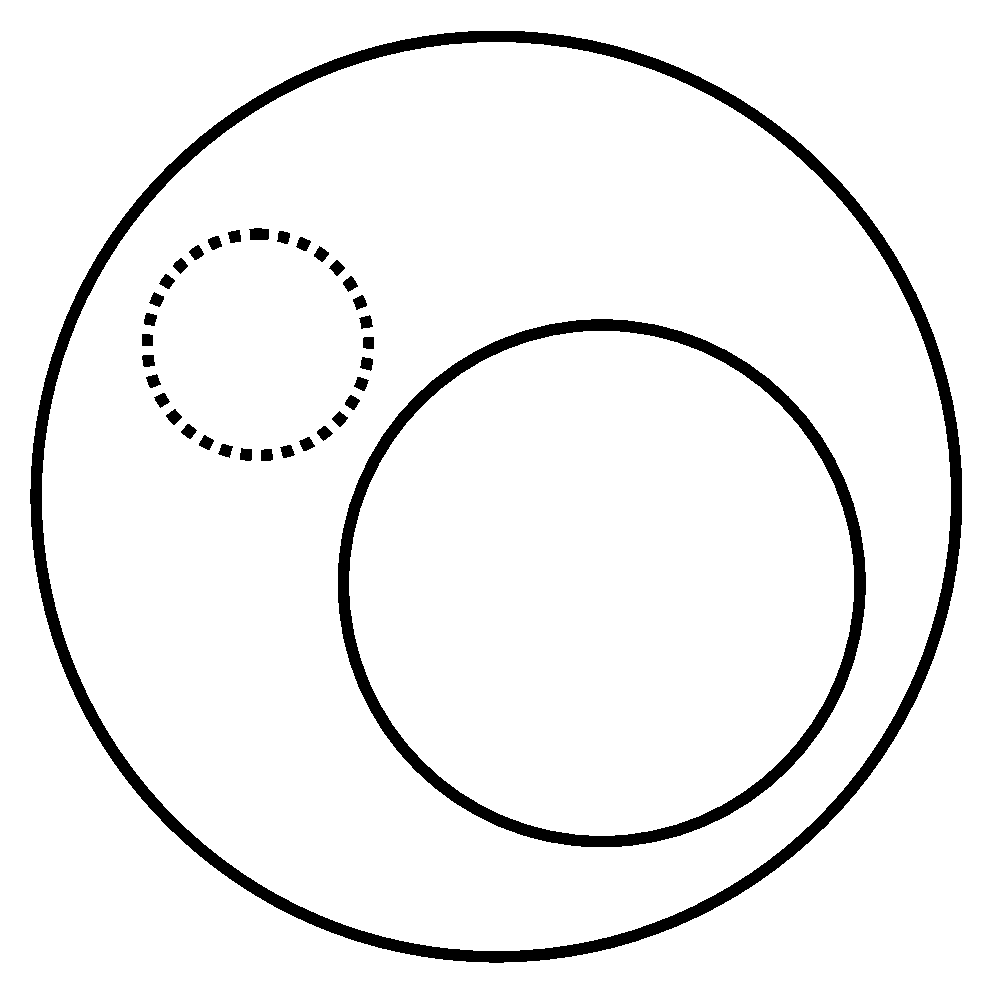
\includegraphics[width=0.4\textwidth]{logotipo.pdf}
\end{standardfigure}

\section{Objetivos} \label{sec:objetivos}
\lipsum[3-4]

\begin{standardfigure}{Equilíbrio e dualidade da Força.}{fig:dualidade}
    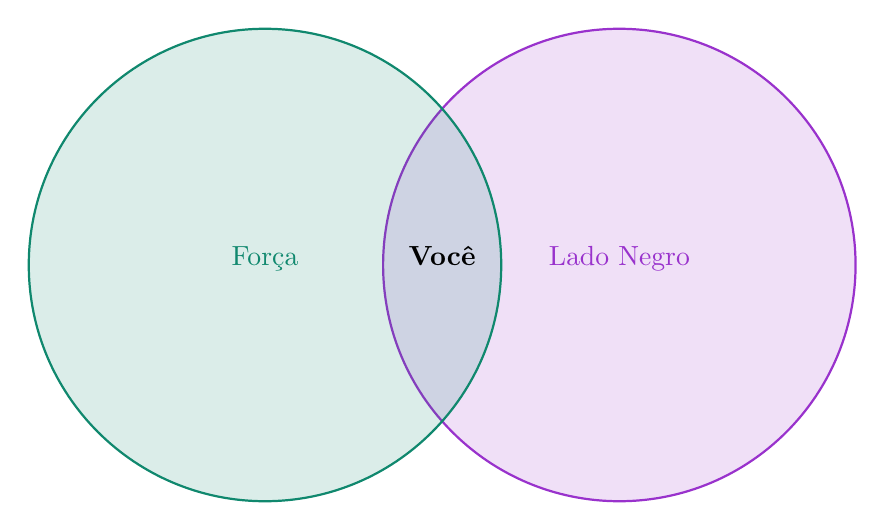
\begin{tikzpicture}
        \filldraw[color=DarkOrchid, fill opacity=0.15, text opacity=1.0, thick] (4.5,0.0) circle (3.0) node[anchor=base]{Lado Negro};
        \filldraw[color=PineGreen, fill opacity=0.15, text opacity=1.0, thick] (0.0,0.0) circle (3.0) node[anchor=base]{Força};
        \node[anchor=base] at (2.25,0.0) {\textbf{Você}};
    \end{tikzpicture}
\end{standardfigure}

\lipsum[5]

\section{Organização da tese} \label{sec:organizacao_tese}
\lipsum[6]